%%%%%%%%%%%%%%%%%%%%%%%%%%%%%%%%%%%%%%%%%%%%%%%%%
\section{Detector Packages}
%%%%%%%%%%%%%%%%%%%%%%%%%%%%%%%%%%%%%%%%%%%%%%%%%
\begin{figure}[!ht]
 \begin{center}
  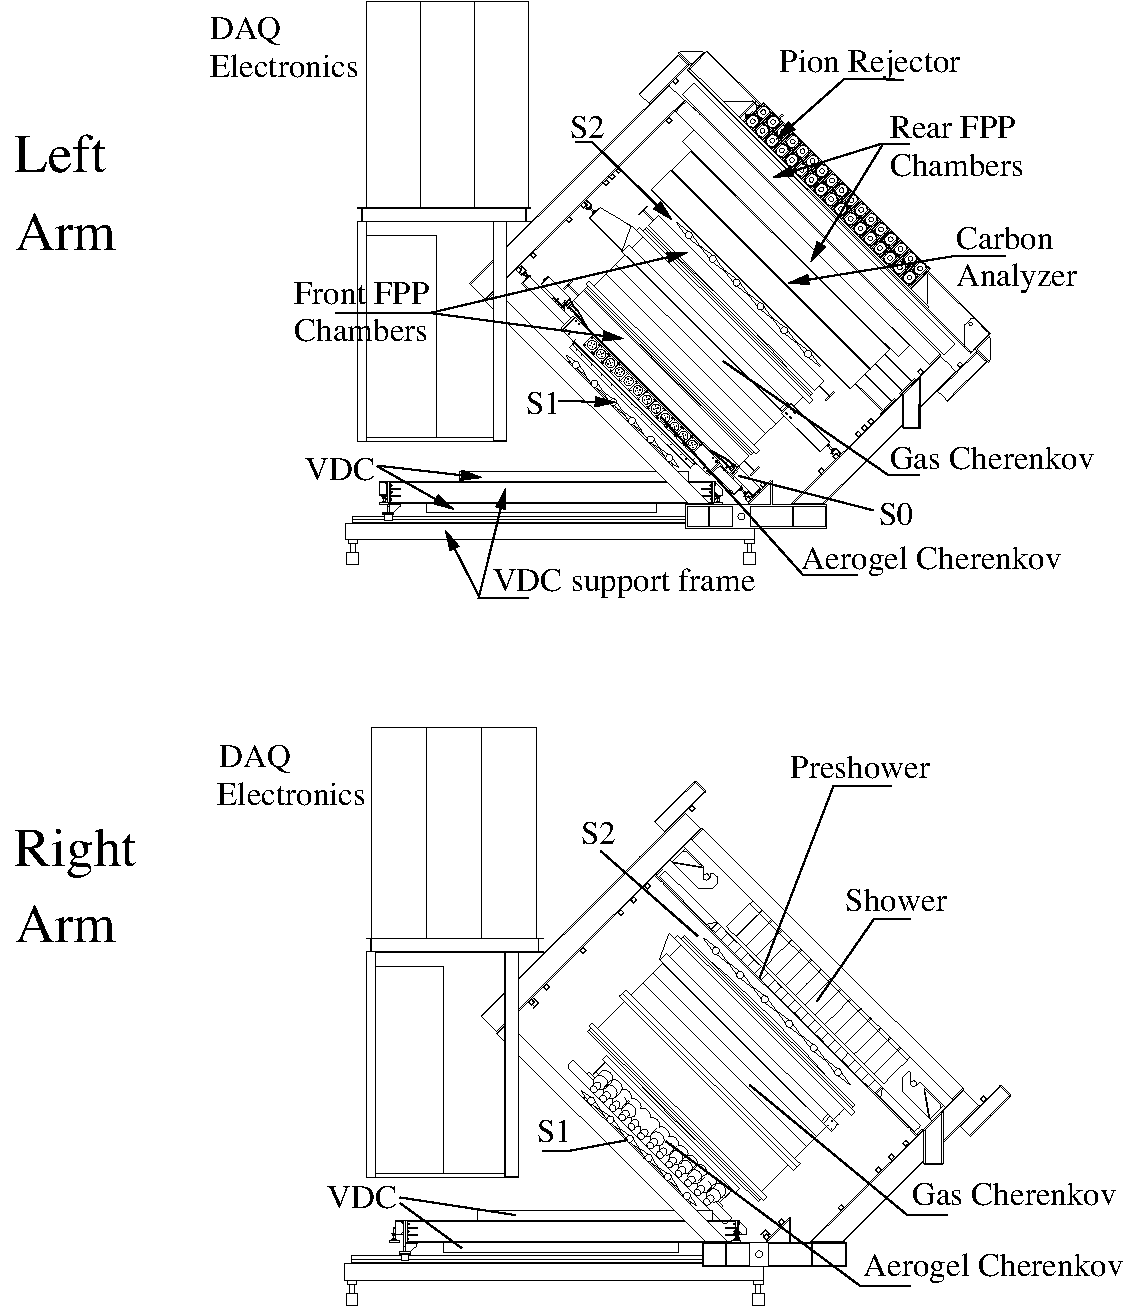
\includegraphics[width=0.7\textwidth]{./figures/halla_jlab/sideview_new}
  \caption[HRS detector stack]{\footnotesize{HRS detector stack, where all detectors available for different experiments are shown. VDCs, S1, S2m, Gas Cherekov detectors and Calorimeters were installed in the E08-014. In addition to these standard detectors, a long single-bar scintillator (S0) and an Aerogel \v{C}erenkov detector (AC) are included in each HRS, and a focal plane polarimeter (FPP) is available in HRS-L. S0, AC and FPP were not used during this experiment. Figure is from Ref.~\cite{halla_nim}.}}
  \label{detecor_hut}
 \end{center}
\end{figure}
 
 Particles coming through the HRS are fully characterized by the detector package and their signal outputs are delivered to the front-end electronics to form trigger signals and to be recorded by the data acquisition (DAQ) system. As shown in Fig.~\ref{detecor_hut}, the detector package in each arm includes two vertical drift chambers (VDCs), two scintillator planes (S1 and S2m), a gas \v{C}erenkov detector (GC), and a calorimeter. 
  
 Signals from VDCs are converted into digital types by the discriminator cards attached on the VDCs and then sent directly into the front-end of the time-to-digital converters (TDC) on the FastBus crate. For all other detectors, each analog signal from the corresponding photomultiplier tube (PMT) is split into two copies. One is properly delayed through a long cable before it is fed into the front-end of an analog-to-digital converter (ADC), and the other one, at the same time, goes through the discriminator module (DIS). If the amplitude of the analog signal is over the threshold value, a digital signal will be created and further used to form trigger signals or be recorded by the TDC front-end. 
 
 In the following sections, the detectors used in this experiment will be individually introduced.

%%%%%%%%%%%%%%%%%%%%%%%%%%%%%%%%%%%%%%%%%%%%%%%%%
\subsection{Vertical Drift Chambers}
%%%%%%%%%%%%%%%%%%%%%%%%%%%%%%%%%%%%%%%%%%%%%%%%%
\begin{figure}[!ht]
 \begin{center}
  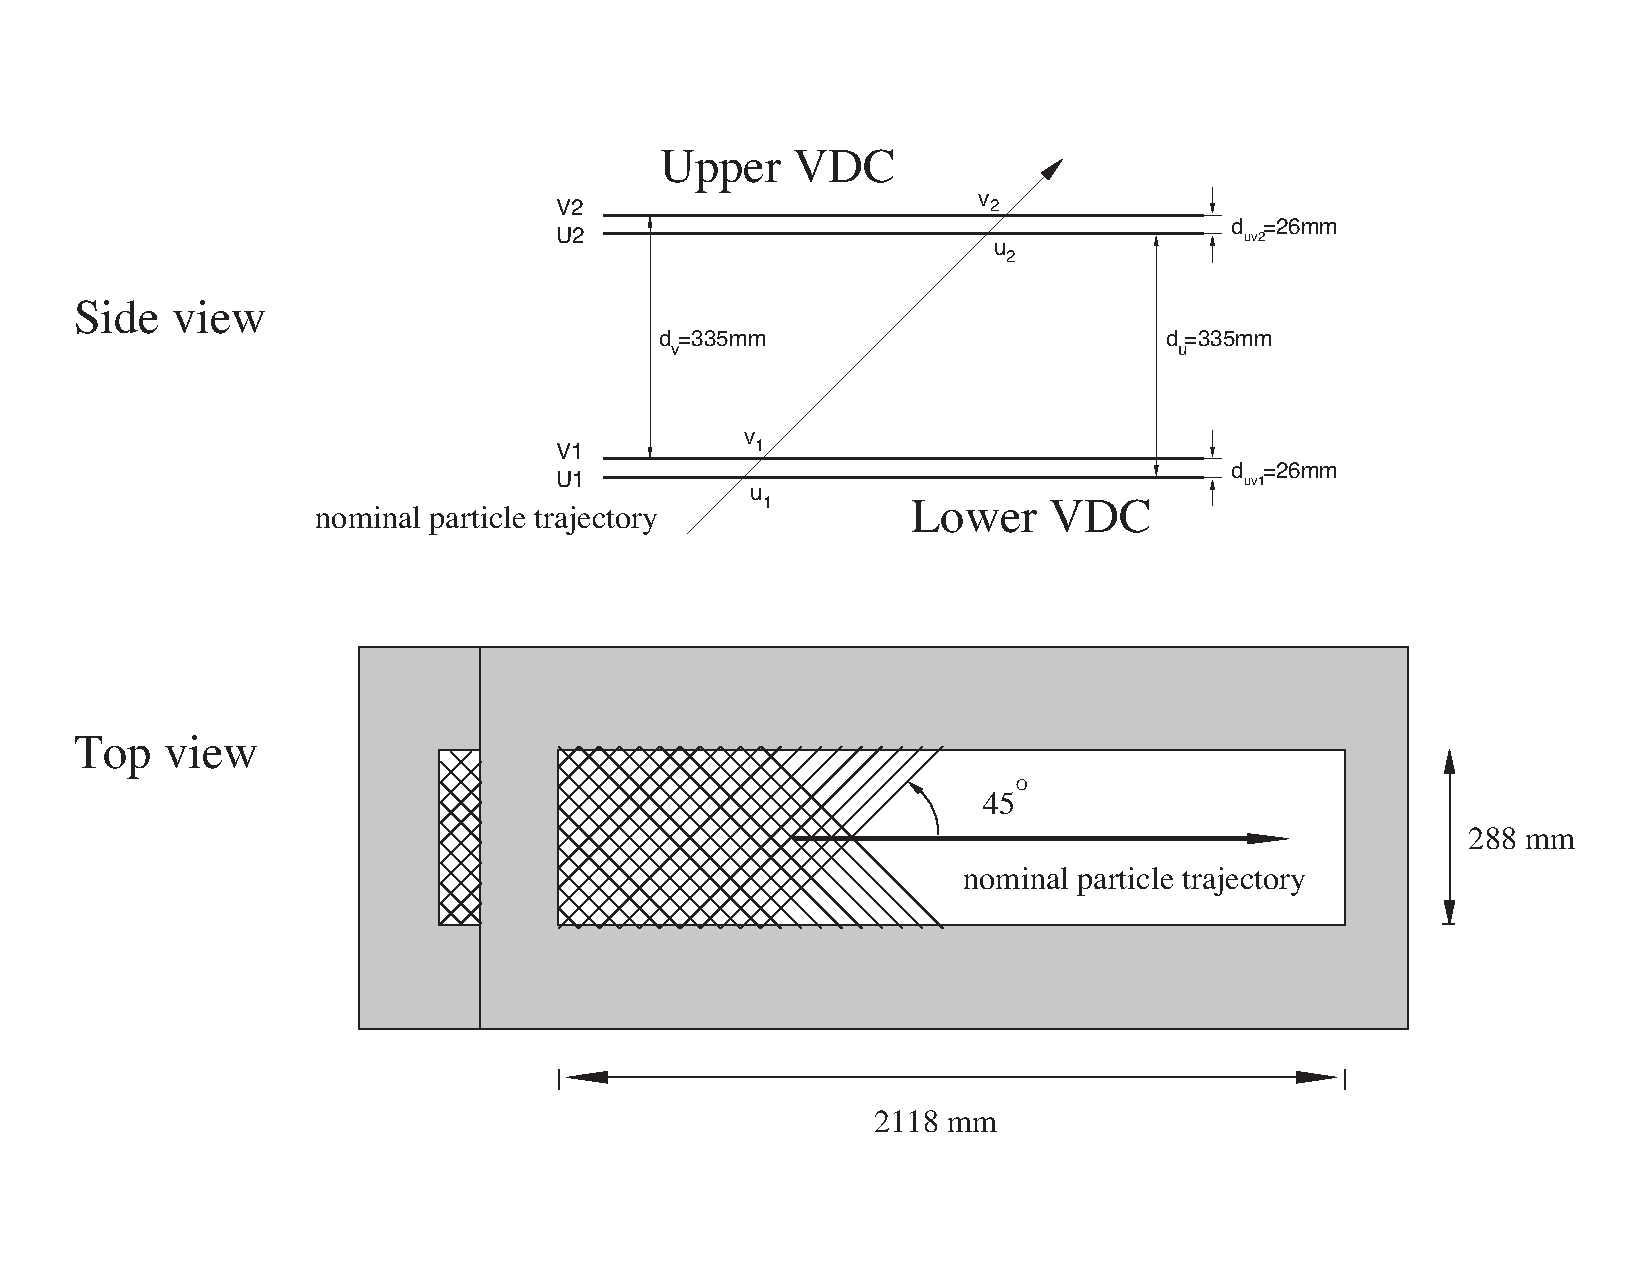
\includegraphics[width=0.6\textwidth]{./figures/vdc/vdc}
  \caption[Layout of Vertical Drift Chambers]{\footnotesize{Layout of Vertical Drift Chambers. Figure is from Ref.~\cite{halla_nim}.}}
  \label{vdc}
 \end{center}
\end{figure}
 The trajectory of a particle after the Q3 exit is tracked by two identical VDCs, which are placed vertically 335~mm apart and lay horizontally $\mathrm{45^{\circ}}$ from the normal particle trajectory~\cite{halla_nim}, as shown in Fig.~\ref{vdc}. There are two wire planes (U and V) in each VDC oriented at $\mathrm{90^{\circ}}$ for one another, and each plane contains 368 wires. Two gold-plated Mylar planes are placed below and above each wire plane, and a high electric field is generated by applying the high voltage (-4~kV) between the wire plane and each Mylar plane. Both VDCs are filled with argon (62\%) and ethane (38\%) with a flow rate of 10~liter/hr. 
 
 When a particle goes through the VDC, the gas molecules are ionized and create a bunch of electrons and ions on the trajectory of the particle. The electrons are accelerated by the high field toward the closest wires, and the signal collected by each wire is amplified and read out by a pre-amplifier TDC card. On average, five sense wires have read-out signals when a particle passes through each wire plane. The exact location where the particle hits on the plane can be reconstructed by those TDC signals. Four locations provided by the four wire planes are used to fit the trajectory of the particle. The position resolution in the focal plane is about 100 $\mathrm{\mu m}$ and the angle resolution is near 100~mrad.

%%%%%%%%%%%%%%%%%%%%%%%%%%%%%%%%%%%%%%%%%%%%%%%%%
\subsection{Scintillator Counters}
%%%%%%%%%%%%%%%%%%%%%%%%%%%%%%%%%%%%%%%%%%%%%%%%%
 Two scintillator planes, S1 and S2m, are placed after the VDCs and separated by 2 m. S1 is composed of 6 overlapping thin plastic paddles, and S2m has 16 smaller paddles. When a charged particle passes through a paddle, it creates light which travels toward both ends of the paddle. A PMT attached to each end of the paddle collects the light and converts it into an analog signal. Scintillators have very fast time-response with very good resolution ($\mathrm{\sim}$30 ns), so their signals are the major source of generating triggers for the DAQ system. The traditional production trigger in Hall-A is generated by requiring both S1 and S2m to be fired within a narrow time window. A detailed discussion of trigger system is given in Section 3.7 and Appendix A.

%%%%%%%%%%%%%%%%%%%%%%%%%%%%%%%%%%%%%%%%%%%%%%%%%
\subsection{Gas \v{C}erenkov Detectors}
%%%%%%%%%%%%%%%%%%%%%%%%%%%%%%%%%%%%%%%%%%%%%%%%%
\begin{figure}[!ht]
 \begin{center}
  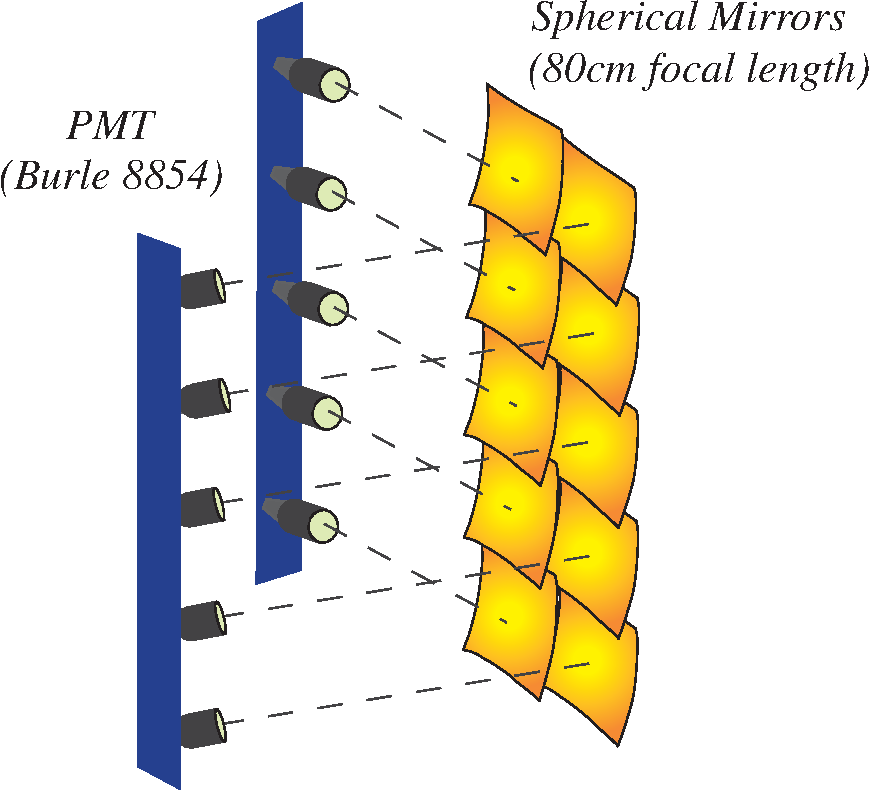
\includegraphics[width=0.6\textwidth]{./figures/cer/cerenkov_design}
  \caption[Design of the gas \v{C}erenkov detector]{\footnotesize{Design of the gas \v{C}erenkov detector. Ten spherical mirrors were carefully arranged to collect the \v{C}erenkov light and focus it into their corresponding PMTs.}}
  \label{gc_pmt}
 \end{center}
\end{figure}
 A high energy charged particle radiates \v{C}erenkov light when it travels in a medium with its speed faster than that of light. The basic mechanism of \v{C}erenkov radiation is that atoms along the track of the particle are polarized and become dipoles, and the variation of these dipole moments emits electromagnetic light\cite{R_Bock}. 
 
 The angle between the direction of \v{C}erenkov light and the track of the charged particle is given by:
\begin{equation}
 cos \theta = \frac{1}{\beta n},
\end{equation}
where $n$ is the index of reflection of the medium. $\beta=v/c$ where $v$ is the charged particle's velocity in the medium and $c$ is the speed of light. The velocity-dependence property of \v{C}erenkov radiation provides an effective tool to discriminate particles with different masses, since the momentum threshold to emit \v{C}erenkov light depends on the mass of the particle:
\begin{equation}
 P_{threshold} = \frac{mc}{\sqrt{n^{2}-1}}.
\end{equation}

 A gas \v{C}erenkov detector (GC), made up of a steel box with thin entry and exit window, is mounted between S1 and S2m on each HRS. Within the box ten light-weight spherical mirrors with very small thickness (0.23~$\mathrm{g\cdot cm^{-2}}$) are positioned in a 2 (horizontal) $\times$ 5 (vertical) array, as shown in Fig.~\ref{gc_pmt}. These mirrors are carefully arranged to efficiently reflect and focus the \v{C}erenkov light on the associated ten PMTs.
 
 The GC box is filled with atmospheric pressure $\mathrm{CO_{2}}$, which gives the index of refraction to be 1.00041. The momentum threshold for electrons to radiate \v{C}erenkov light in this detector is about 18 MeV/c, while the threshold for pions is as high as 4.9 GeV/c. Since the momentum coverage of HRS is from 0.5 GeV/c to 4.3 GeV/c, only electrons can emit \v{C}erenkov light in the detectors. Pions may still be able to produce signals in the GC when they interact with the gas and create low-energy electrons, i.e. $\mathrm{\delta}$-electrons~\cite{pdg}. However, the probability of such process is relatively low and the amplitude of the signal is comparable to the background signal. The path length of the GC on HRS-L is 80~cm which yields an average of 7 photon-electrons, while on HRS-R, the path length for the GC is 130~cm, leading to 12 photon-electron on average~\cite{halla_nim}. The design of GCs provides an excellent electron detection with efficiencies normally above 99\%.

The signal from each PMT is amplified 10 times by an amplifier and divided into two copies. One copy is directly sent to the front-end ADC for offline analysis. The other copy is further split into two pieces, where one is converted into a digital signal and sent to the TDC, while the other one is added together with the similar signals from the other 9 PMTs. The sum of the ten signals is then converted into a digital signal which is used for the design of online triggers, such as the efficiency triggers. During the E08-014, GCs were also included in the production triggers to suppress pion events during the data recording.

%%%%%%%%%%%%%%%%%%%%%%%%%%%%%%%%%%%%%%%%%%%%%%%%%
\subsection{Lead Glass Calorimeters}
%%%%%%%%%%%%%%%%%%%%%%%%%%%%%%%%%%%%%%%%%%%%%%%%%
\begin{figure}[!ht]
 \begin{center}
  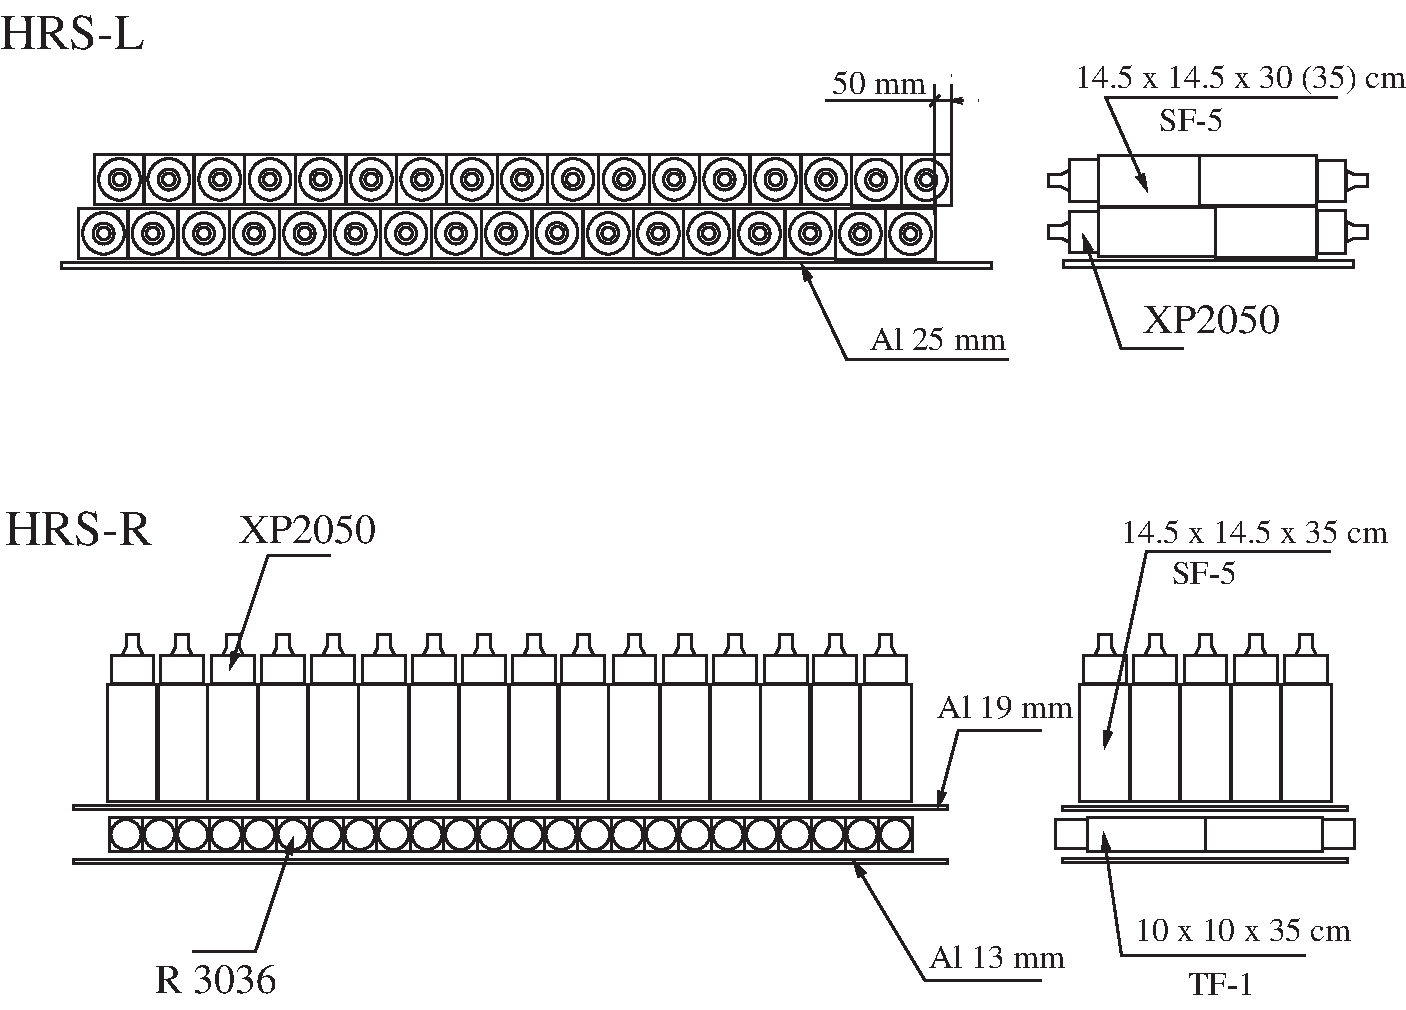
\includegraphics[width=0.7\textwidth]{./figures/calo/ShowerBoth}
  \caption[Schematic layout of calorimeters in HRS-L and HRS-R]{\footnotesize{Schematic layout of calorimeters in HRS-L and HRS-R. Figure is from Ref.~\cite{halla_nim}.}}
  \label{shower}
 \end{center}
\end{figure}

 In each HRS, a calorimeter is placed behind S2m for the energy measurement of charged particles. Each calorimeter is composed of two layers of lead glass blocks and associated PMTs (Fig.~\ref{shower}). The gaps between blocks in the first layer are covered by the blocks in the second layer. The two layers of the calorimeter in HRS-L are called Pion-Rejector-1 (PRL1) and Pion-Rejector-2 (PRL2), respectively, and each layer consists of two columns of 17 lead glass blocks. In HRS-R, the first layer of the calorimeter, also named as PreShower (PS), is formed by two columns of 24 lead glass blocks, while the second layer, called Shower (SH), has five columns of 16 lead glass blocks. 

 When propagating through the dense material, a high energy charged particle loses its energy exclusively through Bremsstrahlung radiation. The emitted photons sequentially create electron-positron pairs which generate secondary Bremsstrahlung radiation. Along the path in the material, an electromagnetic cascade is developed in the direction of incident particle. At the GeV energy scale, only electrons are able to develop such a cascade in the HRS calorimeter. Since heavier particles require a much longer path length, the calorimeter provides a useful substantial particle identification in addition to the GC. PS and SH are arranged to be a total absorber, while PRL1 and PRL2 still provide powerful capability of electron identification even though they don't form a total absorber.
